\documentclass[12pt]{article}
\usepackage{amsmath, amssymb, latexsym, amsthm}
\usepackage{tikz}
\usetikzlibrary{arrows}
\usetikzlibrary{patterns}

\begin{document}

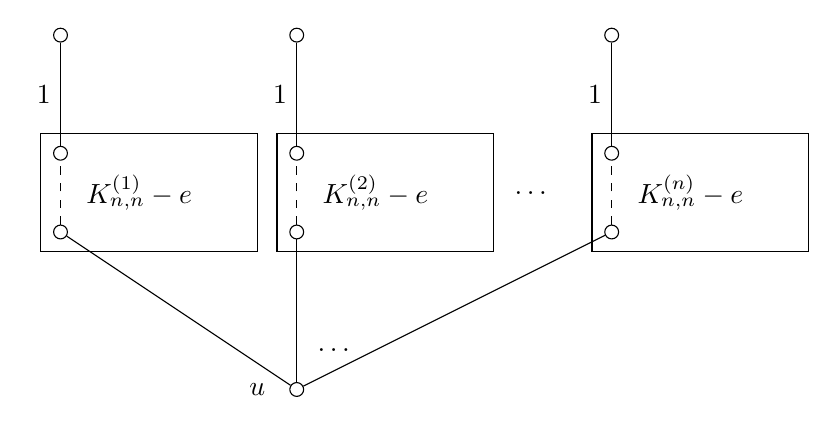
\begin{tikzpicture}[scale=0.5]
	\tikzset{vertex/.style = {shape=circle,draw,
												inner sep=0pt, minimum width=5pt}}
	\tikzset{edge/.style = {-,> = latex'}}
	% vertices
	
	\node[vertex] (u) at  (0, -2) {};
	\node at (-1,-2) {$u$};
	\node[vertex] (x_1) at  (-6, 2) {};
	\node[vertex] (x_2) at  (-6, 4) {};
	\node[vertex] (x_3) at  (-6, 7) {};
	\node[vertex] (y_1) at  (0, 2) {};
	\node[vertex] (y_2) at  (0, 4) {};
	\node[vertex] (y_3) at  (0, 7) {};
	\node[vertex] (z_1) at  (8, 2) {};
	\node[vertex] (z_2) at  (8, 4) {};
		\node[vertex] (z_3) at  (8, 7) {};

	
	%edges
	\draw[dashed] (x_1) to node [] {}  (x_2);
	\draw[edge] (x_2) to node [midway,left] {$1$} (x_3);
	\draw[edge] (y_2) to node [midway,left] {$1$} (y_3);
	\draw[dashed] (y_1) to node [] {}  (y_2);
	\draw[edge] (z_2) to node [midway,left] {$1$} (z_3);
	\draw[dashed] (z_1) to node [] {}  (z_2);
	\draw[edge] (u) to node [] {}  (x_1);
		\draw[edge] (u) to node [] {}  (y_1);
	\draw[edge] (u) to node [] {}  (z_1);
	
\draw [draw=black] (-6.5,4.5) rectangle (-1,1.5);
\node at (-4,3) {$K^{(1)}_{n,n}-e$};
\draw [draw=black] (-0.5,4.5) rectangle (5,1.5);
\node at (2,3) {$K^{(2)}_{n,n}-e$};
\draw [draw=black] (7.5,4.5) rectangle (13,1.5);
\node at (10,3) {$K^{(n)}_{n,n}-e$};

\node at (6,3) {$\dots$};
\node at (1,-1) {$\dots$};


	

%
\end{tikzpicture}

\end{document}